\documentclass[12pt,a4paper]{article}
\usepackage{fontspec}
\usepackage{polyglossia}\setdefaultlanguage{russian}
\setmainfont{DejaVu Serif}\setsansfont{DejaVu Sans}\setmonofont{DejaVu Sans Mono}
\usepackage{amsmath,amssymb,booktabs,graphicx,hyperref,listings,geometry}
\geometry{margin=2.2cm}
\lstset{basicstyle=\ttfamily\scriptsize,breaklines=true,numbers=left,numberstyle=\tiny,frame=single,language=Python,keywordstyle=\color{blue},commentstyle=\color{gray}}
\usepackage{xcolor}
\newcommand{\rc}{r_{\mathrm{crit}}}
\title{Исследование обобщённой дискретной модели\\Вариант 1, $k=4$}
\author{Выполнила: Власенко Ирина Владимировна\\Группа: ИММиКН ПМИ-2.2, номер в списке $k=4$}
\date{28 октября 2026 г.}
\begin{document}\maketitle\tableofcontents\newpage

\section{Постановка задачи и смысл модели}
Исследуется отображение варианта 1 при $k=4$:
\begin{equation}x_{n+1}=r x_n\Bigl(1-\frac{x_n+kx_n^2}{1+k}\Bigr)\ \xrightarrow{k=4}\ f(x)=r x\Bigl(1-\frac{x+4x^2}{5}\Bigr)=\frac r5\,(5x-x^2-4x^3).\label{eq:f}\end{equation}
Величина $x_n$ --- нормированная плотность популяции в поколении $n$, $r>0$ --- скорость роста при малой плотности ($f'(0)=r$), слагаемое $\frac{x+kx^2}{1+k}$ описывает саморегуляцию плотностью, а $k$ определяет её нелинейность; при $k=0$ получается классическое логистическое отображение $rx(1-x)$. Нормировка выбрана так, что $f(1)=0$. Максимум $f$ достигается в точке $c=\frac{\sqrt{61}-1}{12}\approx0{,}5675$ и равен $f(c)\approx0{,}3569\,r$, поэтому отрезок $[0,1]$ инвариантен при $r\le r_{\max}=1/0{,}3569\approx2{,}802$; именно поэтому диапазон $r\in[1;2{,}8]$ используется на диаграмме.

\section{Аналитическое исследование}
\subsection{Неподвижные точки}
Из $f(x)=x$ получаем $x\bigl[r\bigl(1-\frac{x+4x^2}{5}\bigr)-1\bigr]=0$, откуда
\begin{equation}x_1^*=0,\qquad 4x^2+x+\frac5r-5=0\ \Rightarrow\ x^*_\pm=\frac{-1\pm\sqrt{81-80/r}}{8}.\label{eq:fix}\end{equation}
Корень $x^*_-<0$ не имеет физического смысла (отрицательная плотность). Корень $x^*_+>0$ существует при $r>1$. Проверка подстановкой: из $r\bigl(1-\frac{x+4x^2}5\bigr)=1$ получается ровно $4x^2+x+5/r-5=0$, то есть $f(x^*_+)=x^*_+$. Например, при $r=1{,}8$: $x^*_+=\frac{-1+\sqrt{36{,}556}}8\approx0{,}6308$.

\subsection{Устойчивость}
Производная $f'(x)=\frac r5(5-2x-12x^2)$. Для нуля $f'(0)=r$: точка $0$ устойчива при $0<r<1$, при $r>1$ неустойчива. Для $x^*_+$ из $r=\frac5{5-x^*-4x^{*2}}$ следует
\begin{equation}f'(x^*_+)=1-\frac{r\,x^*(1+8x^*)}{5}.\label{eq:fp}\end{equation}
Поскольку $x^*>0$, всегда $f'(x^*_+)<1$, поэтому условие $|f'|<1$ сводится к $f'(x^*_+)>-1$, т.е. $r\,x^*(1+8x^*)<10$. Левая часть возрастает по $r$ (растут и $r$, и $x^*(r)$), следовательно существует единственное $\rc$, и
\begin{equation}x^*_+\ \text{устойчива}\iff 1<r<\rc;\qquad x_1^*\ \text{устойчива}\iff0<r<1.\label{eq:stab}\end{equation}

\subsection{Критическое значение параметра}
Условие $f'(x^*_+)=-1$ даёт $5-2x-12x^2=-(5-x-4x^2)$, т.е.
\begin{equation}16x^2+3x-10=0,\quad x_{\rm crit}=\frac{\sqrt{649}-3}{32}\approx0{,}70236,\quad \rc=\frac5{5-x_{\rm crit}-4x_{\rm crit}^2}\approx2{,}1511.\label{eq:rc}\end{equation}
Проверка: $f'(x_{\rm crit})=-1$, при $r<\rc$ имеем $f'>-1$, а при переходе через $\rc$ производная становится меньше $-1$: это бифуркация удвоения периода. Общий случай: $f'(x^*)=-1\iff4kx^2+3x-2(1+k)=0$; при $k=0$ получаем $x^*=2/3$, $\rc=3$ --- классическое значение для $rx(1-x)$.

\subsection{Цикл периода 2}
Цикл --- пара $x_1\ne x_2$, $f(x_1)=x_2$, $f(x_2)=x_1$; она удовлетворяет $f(f(x))=x$. Так как $f$ кубический, $f\circ f$ имеет степень 9. Полином $f(f(x))-x$ делится на $f(x)-x$ без остатка (проверено в \texttt{sympy}): $f(f(x))-x=(f(x)-x)\,Q(x)$, $\deg Q=6$. Таким образом, для данной модели уравнение цикла --- \emph{шестой} степени, а не квадратное (утверждение методических указаний о квадратном уравнении верно для квадратичных $f$, но не для кубической модели варианта 1).

Тем не менее уравнение решается аналитически через симметрические функции $s=x_1+x_2$, $p=x_1x_2$. Складывая и вычитая уравнения цикла (и деля разность на $x_1-x_2\ne0$), при $f=ax-bx^2-cx^3$, $a=r$, $b=r/5$, $c=4r/5$:
\begin{equation}a-bs-c(s^2-p)=-1,\qquad (a-1)s-b(s^2-2p)-cs(s^2-3p)=0.\end{equation}
Из первого уравнения $p=\frac{4s^2+s-5}4-\frac5{4r}$; подстановка во второе даёт кубическое уравнение
\begin{equation}16r\,s^3+8r\,s^2-(19r+40)\,s-5(r+1)=0.\label{eq:cubic}\end{equation}
Точки цикла --- корни $t^2-st+p=0$, они вещественны и различны при $D=s^2-4p>0$. Из трёх корней (\ref{eq:cubic}) физичный (с $x_{1,2}\in(0,1)$) появляется при $r>\rc$: при $r=2{,}1501$ его нет, при $r=2{,}1521$ есть ($x_{1,2}=0{,}6913;\,0{,}7133$). Два других цикла лежат вне $[0,1]$ (отрицательные $x$).

\emph{Устойчивость:} $|\mu|<1$, $\mu=f'(x_1)f'(x_2)$. Численное решение $\mu=-1$ (бисекция по $r$ вдоль ветви цикла) даёт $r_2\approx2{,}4136$, так что цикл устойчив при $\rc<r<r_2$.

\section{Численные эксперименты}
\subsection{Сходимость к равновесию и к циклу}
На рис.~\ref{fig:ts} показаны $x_n$ при $r=0{,}9\,\rc\approx1{,}936$ (сходимость к $x^*_+\approx0{,}6624$) и при $r=1{,}1\,\rc\approx2{,}366$ (цикл периода 2, $x_{1,2}\approx0{,}5321;\,0{,}8399$); $x_0=0{,}2$.
\begin{figure}[h!]\centering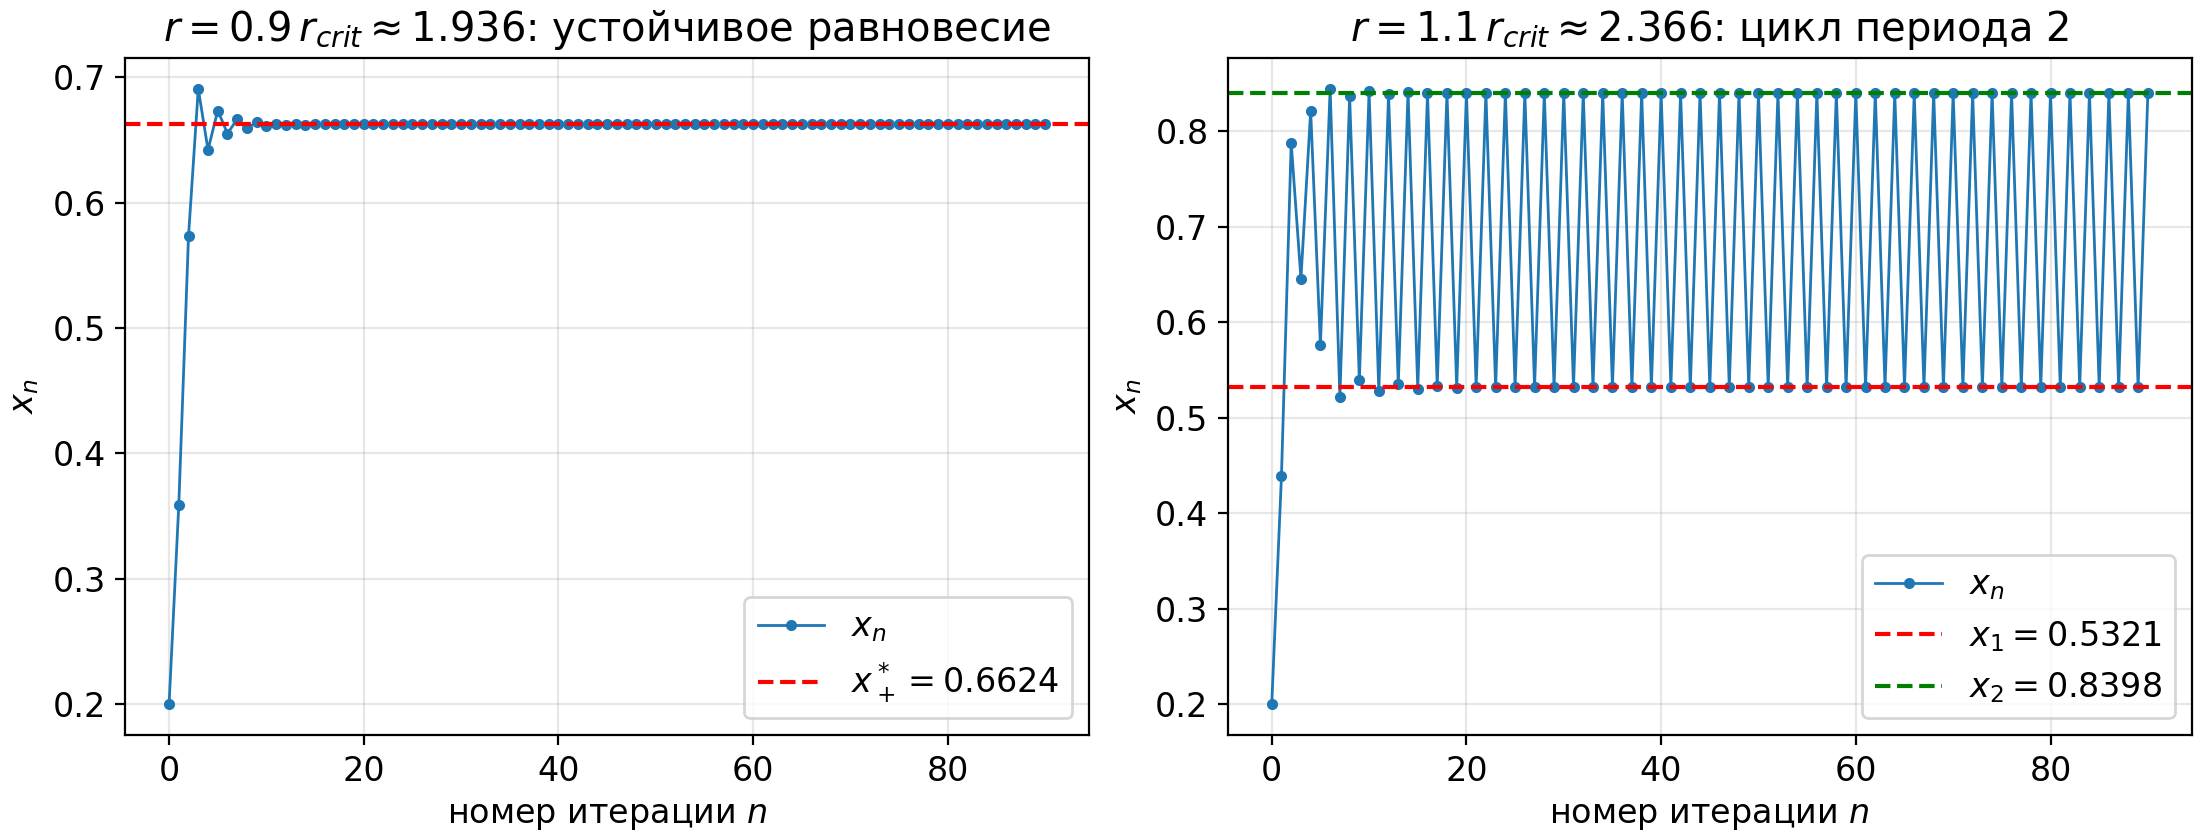
\includegraphics[width=\textwidth]{fig1.png}\caption{Временные ряды при $r=0{,}9\,\rc$ и $r=1{,}1\,\rc$.}\label{fig:ts}\end{figure}

\subsection{Бифуркационная диаграмма}
Для каждого из 3000 значений $r\in[1;2{,}8]$ отбрасывалось 1500 итераций, затем отображалось 250 значений. Первая бифуркация видна при $r\approx\rc=2{,}151$, вторая --- при $r_2\approx2{,}414$; далее наблюдаются каскад удвоений, область хаоса и окно периода 3 при $r\approx2{,}66$ (проверено итерациями: при $r=2{,}66$ орбита $0{,}2283\to0{,}5542\to0{,}9486$ замыкается). Вид диаграммы зависит от сетки по $r$, числа отброшенных итераций и $x_0$.
\begin{figure}[h!]\centering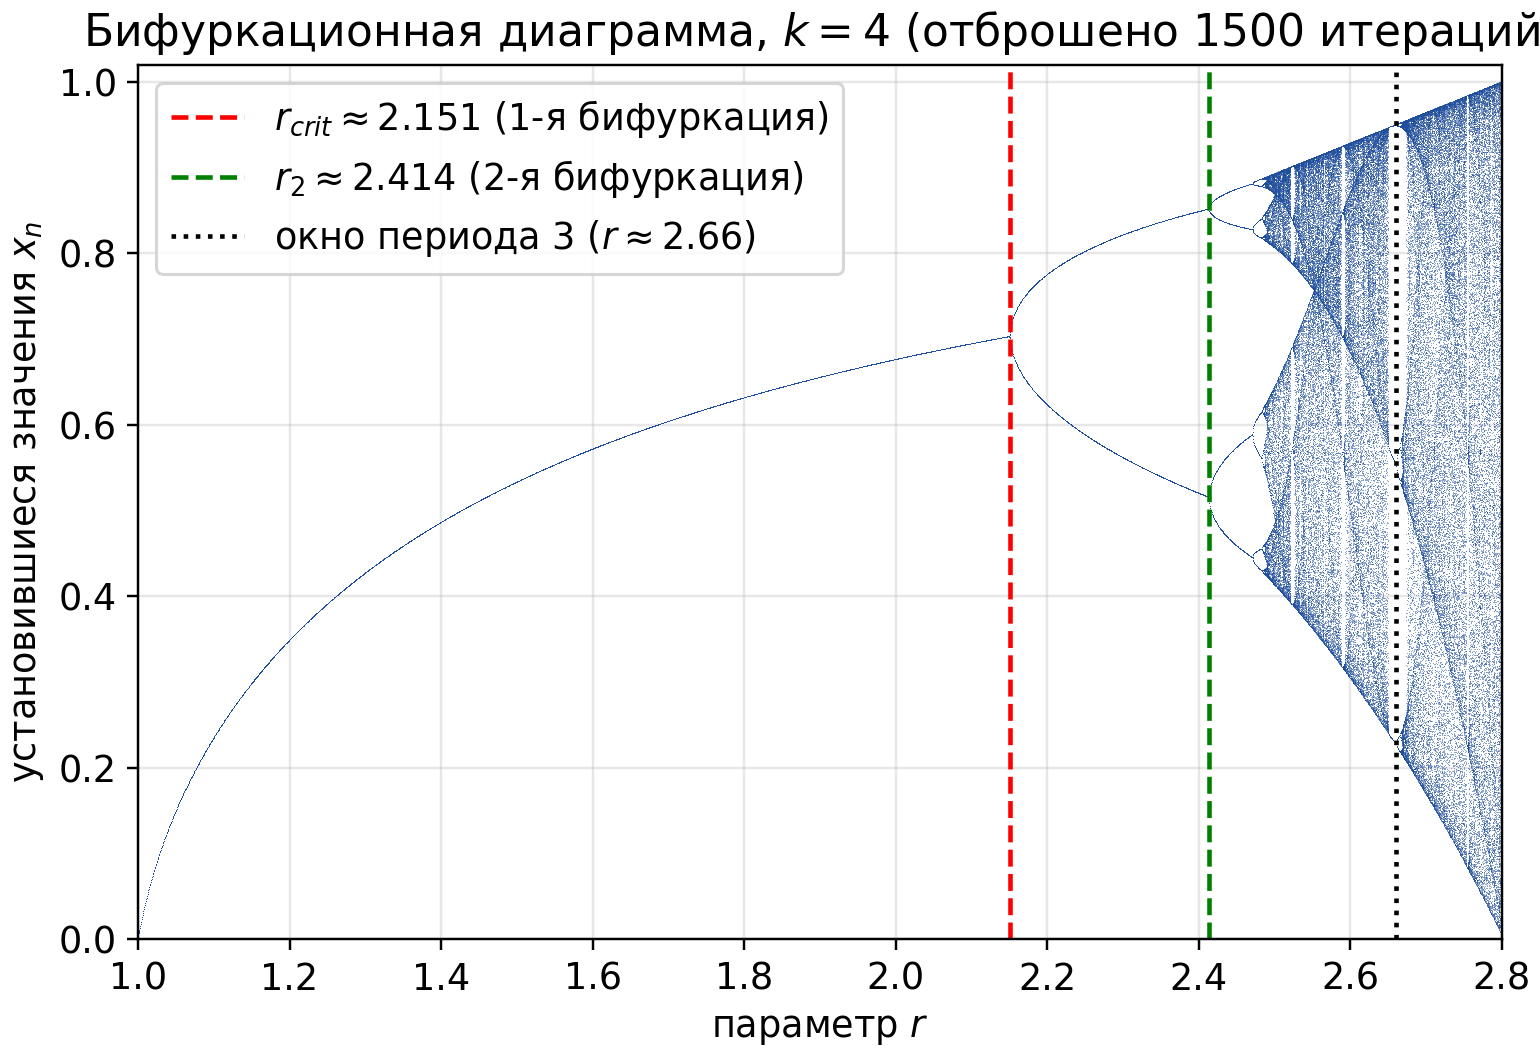
\includegraphics[width=.8\textwidth]{fig2.png}\caption{Бифуркационная диаграмма ($k=4$).}\end{figure}

\subsection{Численное исследование цикла периода 2}
Точки цикла вычислены через (\ref{eq:cubic}); невязка $\varepsilon=\max\{|f(x_1)-x_2|,|f(x_2)-x_1|\}$, мультипликатор $\mu=f'(x_1)f'(x_2)$:
\begin{center}\begin{tabular}{lccccc}\toprule$r$&$x_1$&$x_2$&$\varepsilon$&$\mu$&устойчивость\\\midrule
$1{,}05\,\rc=2{,}2586$&0,58234&0,80527&$8\cdot10^{-15}$&$0{,}210$&да\\
$1{,}1\,\rc=2{,}3662$&0,53204&0,83987&$3\cdot10^{-15}$&$-0{,}621$&да\\
$1{,}2\,\rc=2{,}5813$&0,46388&0,88019&$2\cdot10^{-15}$&$-2{,}405$&нет\\
$2{,}271$&0,57550&0,81024&$1\cdot10^{-14}$&$0{,}116$&да\\\bottomrule\end{tabular}\end{center}
При $r=1{,}2\,\rc$ цикл существует, но неустойчив (так как $r_2/\rc\approx1{,}122$), поэтому требование $|\mu|<1$ для этого значения не выполняется --- система уже перешла к циклу периода 4 и далее. Ветви $x_{1,2}(r)$ и $x^*_+(r)$ показаны на рис.~\ref{fig:br}.
\begin{figure}[h!]\centering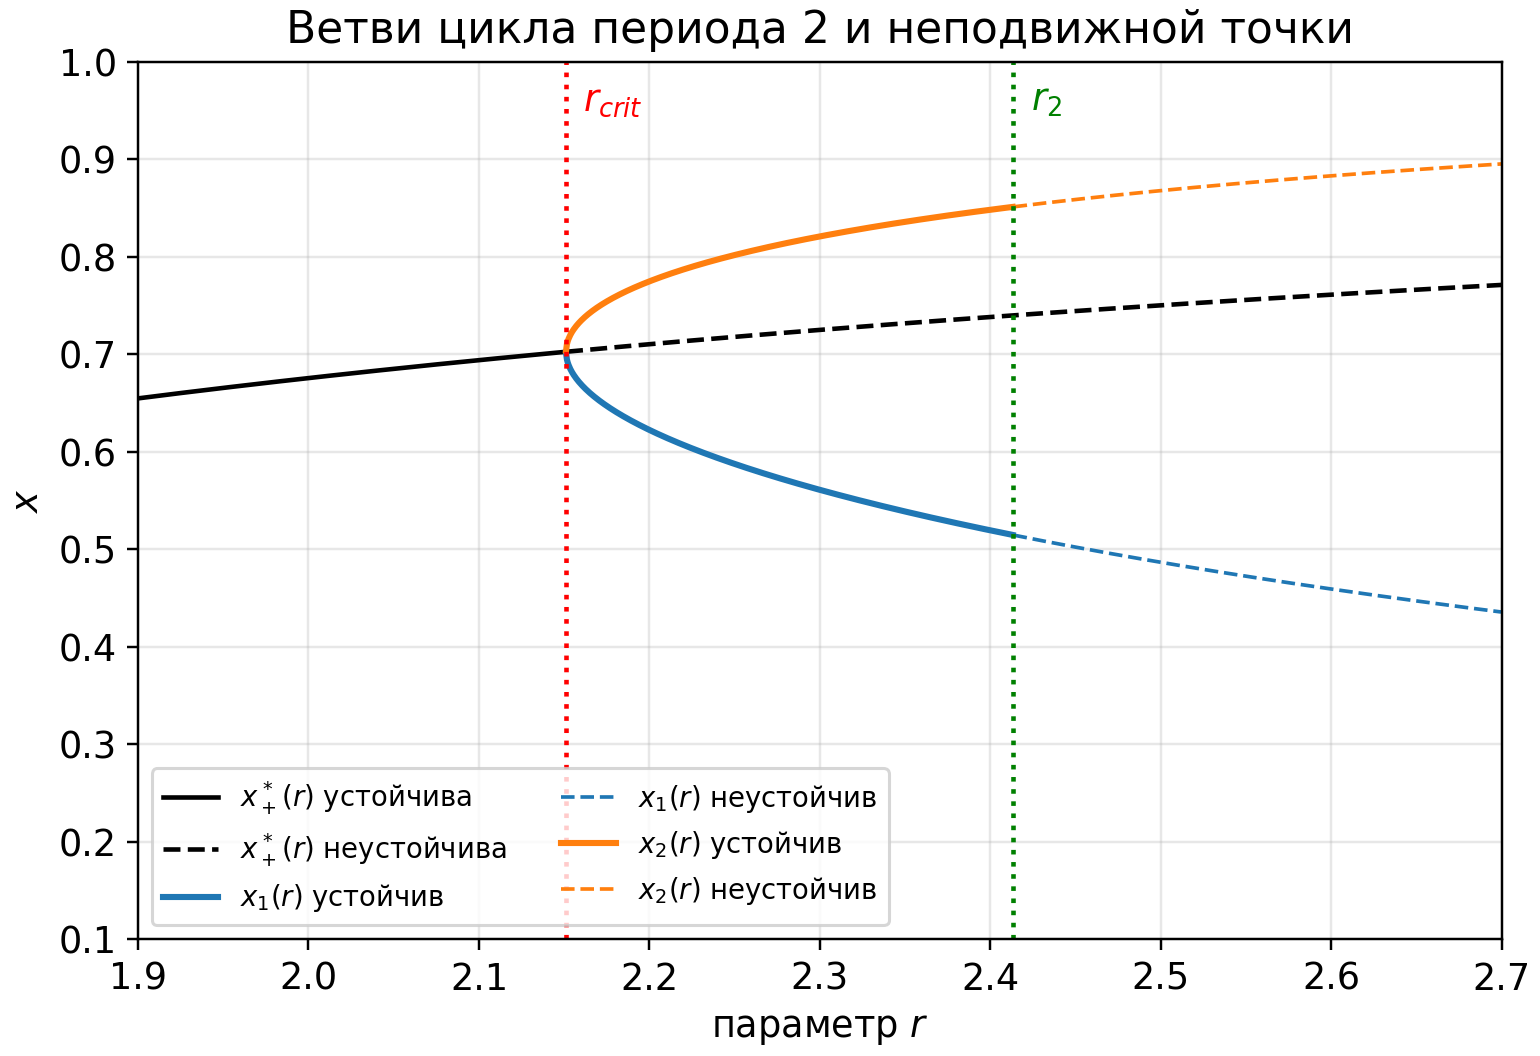
\includegraphics[width=.8\textwidth]{fig3.png}\caption{Ветви цикла периода 2 (сплошная --- устойчивая часть) и неподвижной точки (пунктир --- неустойчивая).}\label{fig:br}\end{figure}

\subsection{Каскад удвоений}
Решая системы $f^{N}(x)=x$, $(f^N)'(x)=-1$ методом Ньютона, получаем точки бифуркаций $\rc=2{,}15108$, $r_2=2{,}41357$, $r_3=2{,}47104$ (4$\to$8), $r_4=2{,}48341$ (8$\to$16). Отношения $\frac{r_2-\rc}{r_3-r_2}\approx4{,}57$, $\frac{r_3-r_2}{r_4-r_3}\approx4{,}64$ приближаются к константе Фейгенбаума $\delta\approx4{,}669$.

\subsection{Хаотический режим, $r=2{,}7$}
Траектория из $10\,000$ итераций после отбрасывания $1000$ (рис.~\ref{fig:ch}). Показатель Ляпунова $\lambda=\langle\ln|f'(x_n)|\rangle\approx0{,}494>0$ (по $2\cdot10^5$ итераций); две траектории с $\Delta x_0=10^{-10}$ расходятся на $0{,}1$ за $\approx40$ итераций. Положительный $\lambda$ и чувствительность к начальным данным подтверждают хаотичность режима.
\begin{figure}[h!]\centering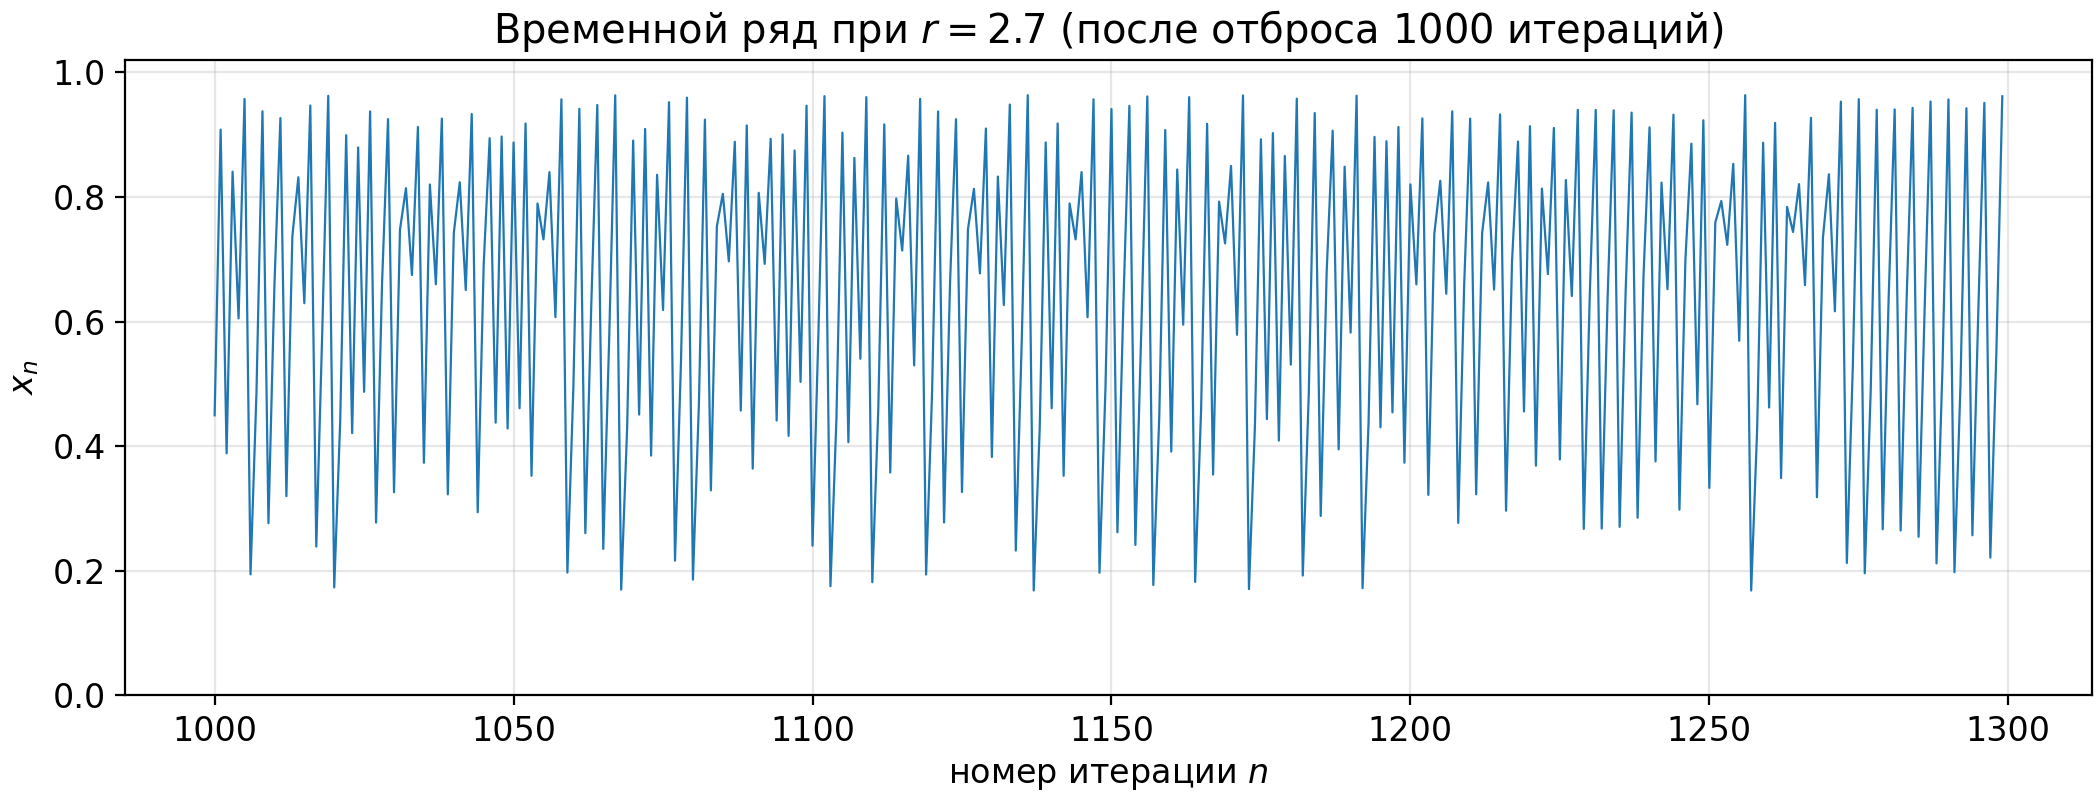
\includegraphics[width=.9\textwidth]{fig4.png}\caption{Временной ряд при $r=2{,}7$.}\label{fig:ch}\end{figure}

Гистограмма (80 бинов, рис.~\ref{fig:hist}) --- эмпирическая инвариантная плотность. \textbf{Запрещённые зоны:} $x<f^2(c)\approx0{,}168$ и $x>f(c)\approx0{,}964$ (значения не выходят за $[f^2(c),f(c)]$, где $c$ --- точка максимума). \textbf{Где больше времени:} пики плотности у границ $f(c)$ и $f^2(c)$ и ступень начиная с $f^3(c)\approx0{,}428$ --- это образы критической точки, характерные для унимодальных отображений; на середине отрезка плотность ниже и приблизительно ровная.
\begin{figure}[h!]\centering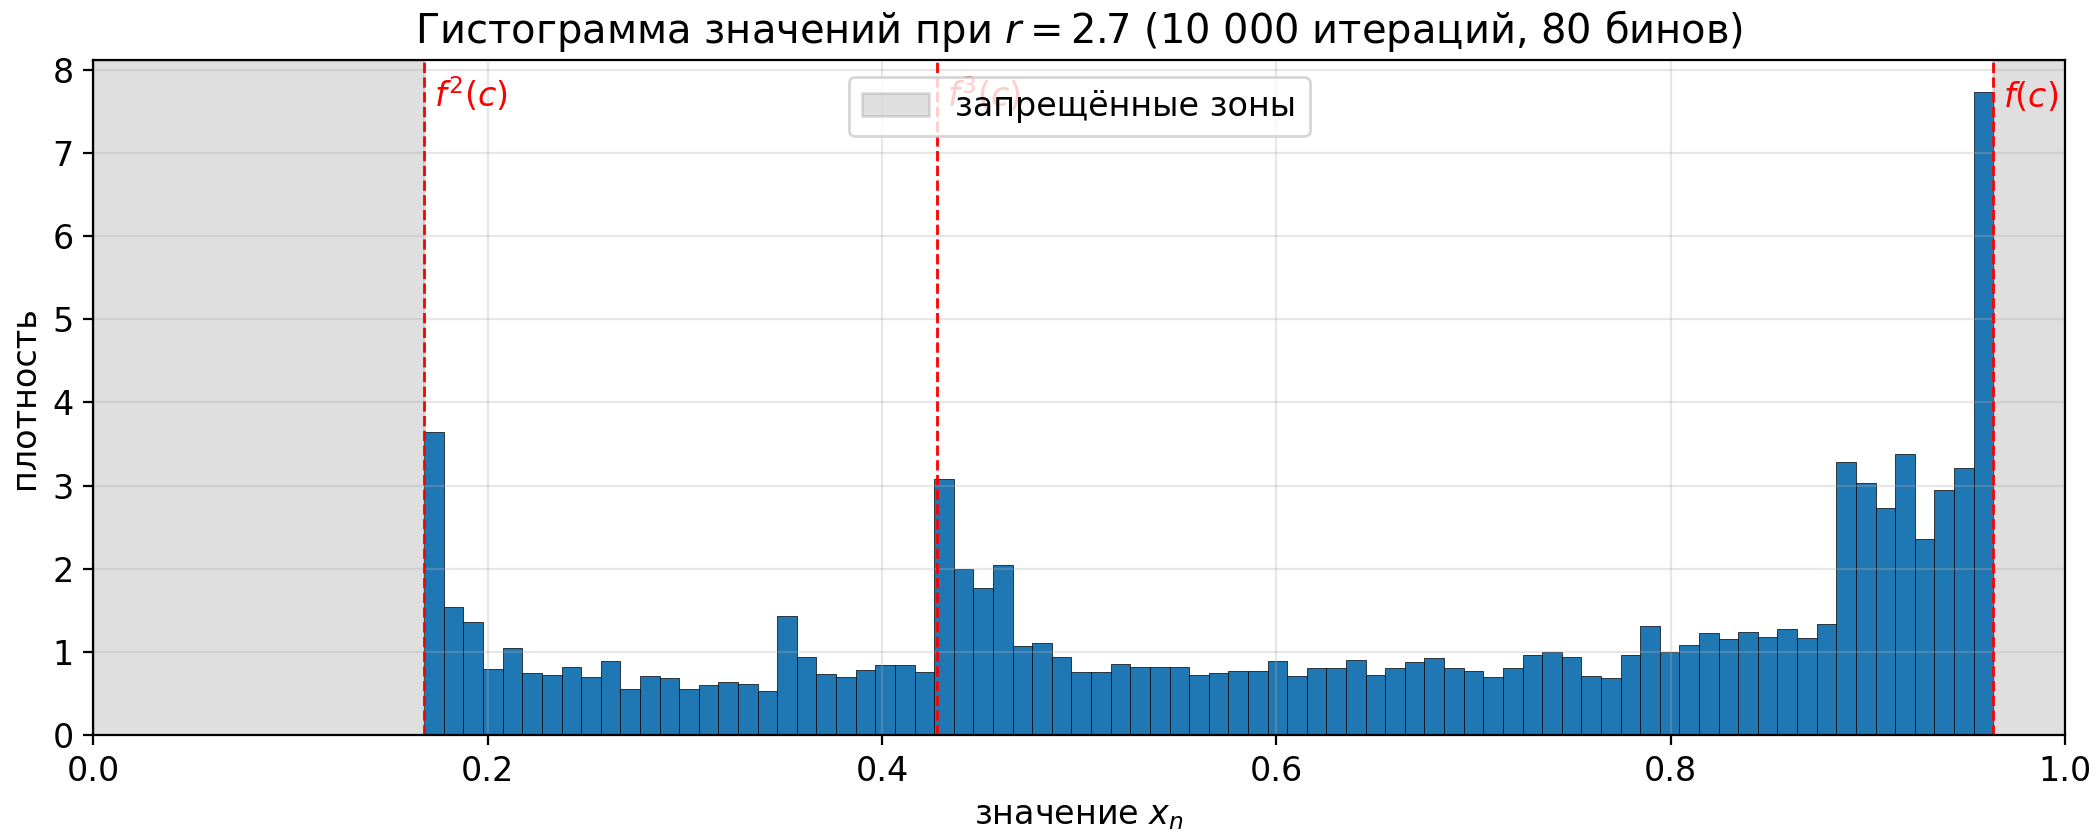
\includegraphics[width=.9\textwidth]{fig5.png}\caption{Гистограмма значений при $r=2{,}7$.}\label{fig:hist}\end{figure}

\section{Литература и сравнение с результатами}
\begin{enumerate}
\item May R.\,M. Simple mathematical models with very complicated dynamics. \emph{Nature}, 261, 459--467, 1976. doi:10.1038/261459a0.
\item May R.\,M., Oster G.\,F. Bifurcations and dynamic complexity in simple ecological models. \emph{The American Naturalist}, 110(974), 573--599, 1976. doi:10.1086/283092.
\item Radwan A.\,G. On some generalized discrete logistic maps. \emph{Journal of Advanced Research}, 4(2), 163--171, 2013. doi:10.1016/j.jare.2012.05.003.
\end{enumerate}
В работах [1,2] показано, что простые нелинейные рекуррентные модели дают каскад удвоений периода и хаос. В [3] введены обобщённые логистические отображения, сводящиеся к классическому, и изучены равновесия, условия устойчивости и бифуркационные диаграммы. Сравнение с нашими результатами: (а) при $k=0$ наша формула $4kx^2+3x-2(1+k)=0$ даёт $\rc=3$ --- классическое значение для $rx(1-x)$, т.е. модель корректно обобщает логистическое отображение; (б) моя диаграмма для $k=4$ показывает первую бифуркацию при $r\approx2{,}151$, т.е. раньше, чем при $k=0$, а сценарий (удвоения $\to$ хаос $\to$ окна периодичности) тот же, что в [1,2]; (в) отношения интервалов $4{,}57$ и $4{,}64$ согласуются с универсальной константой $\approx4{,}669$. Конкретные значения $r$ из [1--3] на данное отображение напрямую не переносятся.

\section{Использование искусственного интеллекта}
Промпты: (1) <<Для модели $x_{n+1}=rx_n(1-(x_n+4x_n^2)/5)$ найди неподвижные точки и покажи преобразования>>; (2) <<Найди производную и выведи $\rc$ из $f'(x^*)=-1$, проверь подстановкой>>; (3) <<Напиши Python-код для временных рядов, бифуркационной диаграммы и гистограммы>>; (4) <<Проверь, что численная пара удовлетворяет $f(x_1)=x_2$, $f(x_2)=x_1$>>.

\textbf{Ошибка 1.} Утверждение, что уравнение цикла периода 2 сводится к квадратному (так сказано и в задании для варианта 1), для кубического $f$ неверно: $\deg Q=6$. Исправление: деление $f(f(x))-x$ на $f(x)-x$ в \texttt{sympy} и сведение к кубическому уравнению (\ref{eq:cubic}) для $s=x_1+x_2$; результат проверен невязкой $\varepsilon\sim10^{-15}$.\\
\textbf{Ошибка 2.} Вывод о хаосе по виду графика недостаточен. Исправление: расчёт показателя Ляпунова $\lambda\approx0{,}494$ и теста чувствительности к $x_0$.\\
ИИ ускорил выкладки и код; формулы, диапазоны $r$ и выводы проверялись вручную и численно.

\section{Заключение}
Найдены $x_1^*=0$ (устойчива при $0<r<1$) и $x^*_+$ (устойчива при $1<r<\rc\approx2{,}1511$); цикл периода 2 рождается при $\rc$ и устойчив до $r_2\approx2{,}4136$; для кубического $f$ он находится из кубического уравнения для $s$ и квадратного для $x_{1,2}$. Каскад удвоений ($r_3\approx2{,}4710$, $r_4\approx2{,}4834$) ведёт к хаосу, при $r=2{,}7$ $\lambda>0$, плотность ограничена отрезком $[0{,}168;0{,}964]$. Результаты качественно согласуются с литературой.

\appendix\section{Листинги программ}
\subsection{Расчёты (\texttt{model\_variant1\_k4.py})}\lstinputlisting{model_variant1_k4.py}
\subsection{Графики (\texttt{figs.py})}\lstinputlisting{figs.py}
\end{document}
